% ─── Slide: Mechanistic insight — MLP vs Attention roles ─────────────────────
\begin{frame}[shrink=20]{Mechanistic Insight: MLP and Attention Play Different Roles}
  \begin{columns}[T]
    \begin{column}{0.50\textwidth}
      \textbf{Finding (v3/v4 ablation):}
      \begin{itemize}
        \item \textbf{MLP diag} $\to$ best \emph{no-ADC} PPL, but wide ADC gap\\
              (better transforms, less robust to ADC noise)
        \item \textbf{Attn diag} $\to$ does \emph{not} improve no-ADC PPL,\\
              but \emph{closes} the ADC gap
        \item \textbf{Inside MLP diag:} \texttt{down\_trans} is the key driver,\\
              not \texttt{up\_gate\_trans}
              (\texttt{down\_proj} sits right before ADC accumulation)
      \end{itemize}

      \vspace{0.15em}
      \textbf{Staged training exploits this:}
      \begin{enumerate}
        \item Stage A (no prop): learn clean MLP diag transforms
        \item Stage B (10 ep, $\alpha{=}0.5$): add attn diag, fine-tune for ADC robustness
      \end{enumerate}

    \end{column}
    \begin{column}{0.46\textwidth}
      % plot_diag_roles.pdf
      \iftrue
        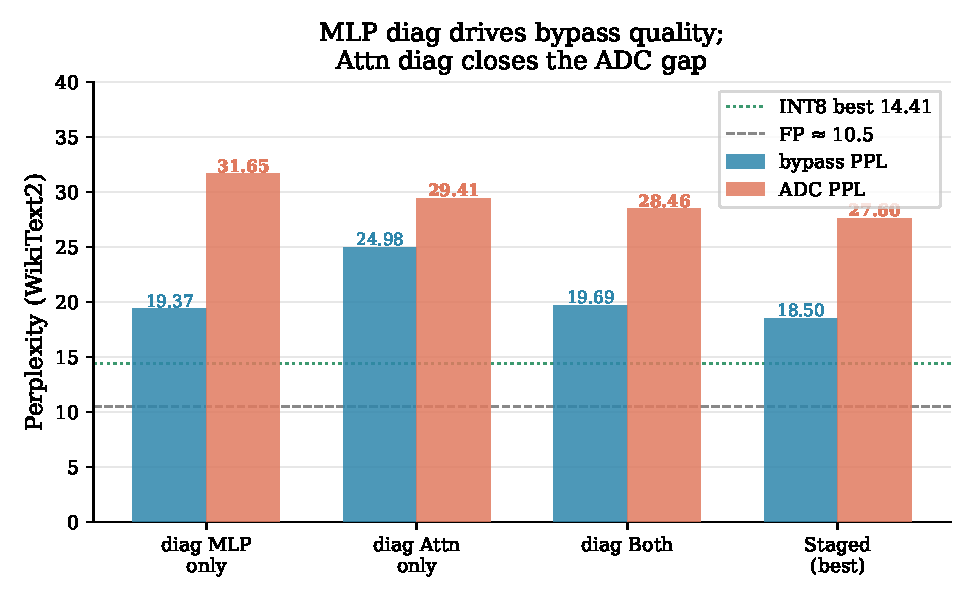
\includegraphics[width=0.95\linewidth]{figs/plot_diag_roles.pdf}
      \else
        \figplaceholder[0.38\textheight]{Grouped bars: \{MLP only, Attn only, Both, Staged\}.
          Two bars per group: no-ADC PPL and ADC PPL.
          Highlight: MLP drives no-ADC PPL, attn drives ADC gap closure.}
      \fi

      \vspace{0.15em}
      % plot_mlp_split_up_down.pdf
      \iftrue
        
\includegraphics[width=0.95\linewidth]{figs/plot_mlp_split_up_down.pdf}
      \else
        \figplaceholder[0.30\textheight]{Grouped bars: \{diag up\_gate, diag down, diag both\}.
          Show no-ADC and ADC PPL.
          Highlight: down\_trans $\gg$ up\_gate\_trans for ADC quality.}
      \fi
    \end{column}
  \end{columns}
\end{frame}
